%!TEX encoding = UTF-8 Unicode

% This file is part of <WORK'S NAME>, <WORK'S BRIEF DESCRIPTION>.
%
% Copyright (C) 2012 Chen-Pang He <jdh8.org>
%
% <WORK'S NAME> is licensed under a
% Creative Commons Attribution-ShareAlike 3.0 Unported License.
%
% You should have received a copy of the license along with this
% work.  If not, see <http://creativecommons.org/licenses/by-sa/3.0/>.

\documentclass[a4paper,12pt]{article}
\usepackage{amsmath,amsthm,amssymb}
\usepackage{CJKutf8}
\usepackage{geometry}
\usepackage{graphicx}
\usepackage[colorlinks,linktoc=page]{hyperref}
\usepackage{pstricks-add}

\setlength{\parindent}{2em}

\begin{document}
\begin{CJK}{UTF8}{bsmi}
\renewcommand{\today}{\number\year~年~\number\month~月~\number\day~日}
\renewcommand{\contentsname}{目錄}
\title{2011 微積分醫學系/牙醫系期中考詳解}
\author{B101100025 何震邦}
\maketitle
\tableofcontents

\section{線性回歸}
In a study of five industrial areas, a researcher obtained these data relating the average number of units of a certain
pollutant in the air and the incidence (per 100\,000 people) of a certain disease:
\begin{center}
\begin{tabular}{c|ccccc}
Units of pollutant&    3&  4&  5&  8& 10\\\hline
Incidence of disease& 48& 52& 58& 70& 96
\end{tabular}
\end{center}
Find the equation of the least-squares line $y=Ax+b$ (to two decimal points [\textit{sic} places.])
\[\textrm{Given that}\; A = \frac{n\sum xy - \sum x \sum y}{n\sum x^2 - (\sum x)^2} \;\textrm{and}\;
                        B = \frac{\sum y - A\sum x}{n}.\]

\paragraph{直接解}
從式子中,我們可以看到,所需要的變數有$n, \sum x, \sum y, \sum x^2, \sum xy$這五項。所以求精確解最有效的方法就是列表。
\begin{center}
\begin{tabular}{ccccc}
      & $x$& $y$& $x^2$& $xy$\\\hline
      &   3&  48&     9&  144\\
      &   4&  52&    16&  208\\
      &   5&  58&    25&  290\\
      &   8&  70&    64&  560\\
      &  10&  96&   100&  980\\\hline
$\sum$&  30& 324&   214& 2162\\
\end{tabular}
\end{center}
事實上,計算機(calculator)上線性回歸的子程式(subroutine)即是依此編寫。因此使用者中途加入、移除資料,計算機可以同步更新。
\begin{center}
\psset{yunit=1mm}
\begin{pspicture}(0,15)(10,100)
\psaxes[Oy=20,Dy=10](0,20)(10,100)
\psdots(3,48)(4,52)(5,58)(8,70)(10,96)
\psline(0,26.32941176)(10,90.44705882)
\end{pspicture}
\end{center}

\section{正弦函數和餘弦函數的導函數}
\subsection{A 卷}
Use the definition of the derivative $\displaystyle f'(x)=\lim_{h\to0}\dfrac{f(x+h)-f(x)}{h}$ to find $\dfrac{d}{dx}\sin x$.

\paragraph{解}
\begin{align*}
\frac{d}{dx}\sin x &= \lim_{h\to0}\frac{\sin(x+h) - \sin x}{h}\\
&= \lim_{h\to0}\frac{\sin x \cos h + \cos x \sin h - \sin x}{h}\\
&= (-\sin x)\left(\lim_{h\to0}\frac{1-\cos h}{h}\right) + (\cos x)\left(\lim_{h\to0}\frac{\sin h}{h}\right)\\
&= \cos x.
\end{align*}

\subsection{B 卷}
Use the definition of the derivative $\displaystyle f'(x)=\lim_{h\to0}\frac{f(x+h)-f(x)}{h}$ to find $\dfrac{d}{dx}\cos x$.

\paragraph{解}
\begin{align*}
\frac{d}{dx}\cos x &= \lim_{h\to0}\frac{\cos(x+h) - \cos x}{h}\\
&= \lim_{h\to0}\frac{\cos x \cos h - \sin x \sin h - \sin x}{h}\\
&= (-\cos x)\left(\lim_{h\to0}\frac{1-\cos h}{h}\right) - (\sin x)\left(\lim_{h\to0}\frac{\sin h}{h}\right)\\
&= -\sin x.
\end{align*}

\section{求曲線上的切線及法線}
\subsection{A 卷}
Find the equation of the tangent line of the curve $y^3 - xy^2 + xy = 3$ [\textit{sic} $-14$] at $(1,-2)$.
\paragraph{解}
\begin{enumerate}
\item 我們已經知道切線通過 $(1,-2)$ 了,所以知道斜率就可以代入點斜式,求出切線方程式。
\item 斜率就是 $dy/dx$,所以不妨在等式兩邊都 apply $d/dx$。
\end{enumerate}

\begin{align*}
y^3 - xy^2 + xy &= -14\\
3y^2 y' - (2xyy' + y^2) + (xy' + y) &= 0\\
(3y^2 - 2xy + x)y' &= y^2 - y\\
y' &= \frac{y^2 - y}{3y^2 - 2xy + x}\\
y'(1,-2) &= \frac{6}{17}.
\end{align*}

所以切線方程式為
\[ y+2 = \frac{6}{17}(x-1). \]

\subsection{B 卷}
Find the equation of the normal line of the curve $y^3 - xy^2 + xy = 3$ [\textit{sic} $-14$] at $(1,-2)$.
\paragraph{解}
解法幾乎與 A 卷相同,唯法線的斜率是切線斜率的 -1 倍。所以法線方程式為
\[ y+2 = \frac{-17}{6}(x-1). \]

\section{有理函數的導函數}
Given $f(x)=\dfrac{x^2 (1-x)^3}{1+x}$, find $f'(2)$.

\paragraph{對數微分法}
\begin{align*}
f(x) &= -x^2 (x-1)^3 (x+1)^{-1}\\
\ln |f(x)| &= 2 \ln |x| + 3 \ln |x-1| - \ln |x+1|\\
\frac{f'(x)}{f(x)} &= \frac{2}{x} + \frac{3}{x-1} - \frac{1}{x+1}\\
f'(x) &= \frac{-x^2 (x-1)^3}{x+1}\left(\frac{2}{x} + \frac{3}{x-1} - \frac{1}{x+1}\right)\\
f'(2) &= \frac{-4}{3}\left(1 + 3 - \frac{1}{3}\right) = \frac{-44}{9}.
\end{align*}

\paragraph{直接法}
\begin{align*}
f(x) &= \frac{-x^2 (x-1)^3}{x+1}\\
f'(x) &= \frac{-2x (x-1)^3 - 3x^2 (x-1)^2}{x+1} + \frac{x^2 (x-1)^3}{(x+1)^2}\\
f'(2) &= \frac{-4 - 12}{3} + \frac{4}{9} = \frac{-44}{9}.
\end{align*}

\section{作圖}
Sketch the graph of $\dfrac{3x^5 - 20x^3 + 1}{32}$ and also mark the absolute extreme points and inflection points at
interval $[-3, 3]$.

\paragraph{解}
因為題目要求反曲點,所以要做到二階導函數。
\begin{align*}
  f(x) &= \frac{3x^5 - 20x^3 + 1}{32}\\
 f'(x) &= \frac{15x^4 - 60x^2}{32}\\
f''(x) &= \frac{15x^3 - 30x}{8}.
\end{align*}

解導函數的零點,找到此函數在 $[-3,3]$ 的臨界點為 $-3, -2, 0, 2, 3$。
\[f(-3)=\frac{-47}{8},\; f(-2)=\frac{65}{32},\; f(0)=\frac{1}{32},\; f(2)=\frac{-63}{32},\; f(3)=\frac{95}{16}.\]

由此可知,最大值在 $(3,5.9375)$ 而最小值在 $(-3,-5.875)$。

解二階導函數的零點,找到此函數可能的反曲點為 $-\sqrt2, 0, \sqrt2$。
\[f(-\sqrt2) = \frac{7\sqrt2}{8} + \frac{1}{32},\; f(0)=\frac{1}{32},\; f(\sqrt2) = \frac{-7\sqrt2}{8} + \frac{1}{32}.\]

所以可能的反曲點座標在 $(-1.414213562,1.268686867)$ 、 $(0,0.03125)$ 和 $(1.414213562,-1.206186867)$。

另外雖然題目並不要求局部極值,不過反正你也求出 $(-2,2.03125)$ 和 $(2,-1.96875)$ 了,不用可惜。而且 $f(x)$ 的零點如果抓不準,%
圖會很醜。所以如果時間允許,找一下 $f(x)=0$ 的根來美化圖形吧!

如下圖,當你已經點出圖上所有題目要求的點,也就是黑點,再加上局部極值,就可大概看出兩根約在 $\pm 2.5$ 附近。當然 0 附近還有一%
個小小的正根,不過那對圖形的美觀沒有影響。

當代電腦、計算機要求多項式的所有根,已經不太適合採用牛頓法(Newton's method)了\footnote{因為牛頓法平均收斂性能為平方收斂%
(quadratic convergence),且不保證能找到根。但是 QR 演算法平均達到立方收斂(cubic convergence),且在最壞情況仍有平方收斂。%
絕對值相近的根,是所有求根演算法的殺手。這當然包括重根、共軛根、相反數根等。}\footnote{QR 演算法只能解多項式的根。當代電腦、%
計算機解非線性方程還是倚靠牛頓法為主。}。然而牛頓法還是比較適合手算,而且比假位法(false position, \textit{regula falsi})和%
二分法(bisection)準。

由牛頓法的公式得
\[x_{n+1} = x_n - \frac{f(x_n)}{f'(x_n)}
          = x_n - \frac{3x_n^5 - 20x_n^3 + 1}{15x_n^4 - 60x_n^2}
	  = \frac{12x_n^5 - 40x^3 + 1}{15x_n^4 - 60x_n^2}.\]

又若其真確根為 $\alpha$,則在第 $n$ 步時,必可在 $x_n$ 與 $\alpha$ 間找到 $\xi_n$ 使得
\[\epsilon_{n+1} = \frac{-f''(\xi_n)}{2f'(x_n)}\:\epsilon_n^2.\]

我們分別以 $\pm 2.5$ 為起始點 $x_0$,發現其實一步就夠準了。第一步移動的距離小於 0.1 ,只比筆跡的寬度厚一些,可見誤差已達 0.01
級,因為牛頓法是平方收斂。所以第二步的誤差基本上是 $10^{-3}$ 級,根本不痛不癢,考試的時候就不要做下去了。

以下我們列出前二步的結果。
\[\begin{aligned}
x_0 &=  2.5 &\Rightarrow x_1 &= \frac{3375}{512} \approx  2.5878 &\Rightarrow x_2 &\approx  2.5783\\
x_0 &= -2.5 &\Rightarrow x_1 &= \frac{-974}{375} \approx -2.5973 &\Rightarrow x_2 &\approx -2.5859.
\end{aligned}\]

\subparagraph{作弊快速法}
我去翻了 GNU C 函式庫的源碼,發現他計算單精度浮點數(\verb|float|)的平方根竟然用二分逼近法。可見對人類而言,精度七位以內的用%
直式開方應該比較快。又因為 1/32 實在小得可憐,在零點附近的斜率又頗大,把常數項 1/32 無視後的誤差根本就不出 0.01。

把常數項無視之後,所求兩根就是 $\sqrt{20/3}$,即 $\sqrt{6.66\dots}$,直式開方得 2.58\dots 就可以去點座標嘍!

\begin{center}
\begin{tabular}{c@{}c@{}c r@{}r@{}r@{\,}r}
 & & &        2&.& 5& 8\\
\hline
2& & &$\surd$ 6&.&66&66\\
2& & &        4& &  &  \\
\hline
4&5& &        2& &66&  \\
 &5& &        2& &25&  \\
\hline
5&0&8&         & &41&66\\
 & & &         & &40&64\\
\hline
 & & &         & & 1&02
\end{tabular}
\end{center}

\subparagraph{原理}
\begin{center}
\begin{tabular}{lc@{} lcl}
        &       &$a$   &+& $b$\\
\hline
$a$     &$\surd$&$(a$  &+& $b)^2$\\
$a$     &       &$a^2$ & &\\
\hline
$2a + b$&       &$2ab$ &+& $b^2$\\
        &       &$2ab$ &+& $b^2$\\
\hline
\hline
\end{tabular}
\end{center}


\begin{center}
\psset{xunit=2}
\begin{pspicture}(-3,-6)(3,6)
\psaxes[labels=none,linecolor=gray](0,0)(-3,-6)(3,6)
\psplot[plotstyle=curve]{-3}{3}{x x mul dup x mul exch 3 mul 20 sub mul 1 add 32 div}
\psdots[linecolor=green](-3,-5.875)(-1.414213562,1.268686867)(0,0.03125)(1.414213562,-1.206186867)(3,5.9375)
\psdots[dotstyle=o](-2.585719992,0)(-2,2.03125)(2,-1.96875)(2.578219675,0);

\uput[  0](-3          ,-5.875      ){\footnotesize 最小值 $\left(-3        ,\dfrac{-47}{ 8}                    \right)$}
\uput[270](-2.585719992, 0          ){\footnotesize 零點   $\left(-2.5857200,0                                  \right)$}
\uput[ 90](-2          , 2.03125    ){\footnotesize 極大值 $\left(-2        ,\dfrac{ 65}{32}                    \right)$}
\uput[  0](-1.414213562, 1.268686867){\footnotesize 反曲點 $\left(-\sqrt2   ,\dfrac{ 7\sqrt2}{8} + \dfrac{1}{32}\right)$}
\uput[270]( 0          , 0.03125    ){\footnotesize 反曲點 $\left( 0        ,\dfrac{  1}{32}                    \right)$}
\uput[225]( 1.414213562,-1.206186867){\footnotesize 反曲點 $\left( \sqrt2   ,\dfrac{-7\sqrt2}{8} + \dfrac{1}{32}\right)$}
\uput[270]( 2          ,-1.96875    ){\footnotesize 極小值 $\left( 2        ,\dfrac{-63}{32}                    \right)$}
\uput[ 90]( 2.578219675, 0          ){\footnotesize 零點   $\left( 2.5782197,0                                  \right)$}
\uput[180]( 3          , 5.9375     ){\footnotesize 最大值 $\left( 3        ,\dfrac{ 95}{16}                    \right)$}
\end{pspicture}
\end{center}

\section{複合函數的導函數}
\subsection{A 卷}
Given $f(x) = \ln(\sec^4 x + \tan^2 x)$, find $f'(\pi/4)$.

\paragraph{解}
\begin{align*}
f(x) &= \ln(\sec^4 x + \tan^2 x)\\
f'(x) &= \frac{4 \sec^4 x \tan x + 2 \sec^2 x \tan x}{\sec^4 x + \tan^2 x}\\
f'\left(\frac{\pi}{4}\right) &= \frac{16 + 4}{4 + 1} = 4.
\end{align*}

\subsection{B 卷}
原文已散佚,$f(x)$ 是從解答重建的。
\begin{align*}
f(x) &= (x^2 + 1)^{\sin x}\\
\ln |f(x)| &= \sin x \ln(x^2 + 1)\\
\frac{f'(x)}{f(x)} &= \cos x \ln(x^2 + 1) + \frac{2x \sin x}{x^2 + 1}\\
f'(x) &= (x^2 + 1)^{\sin x} \left(\cos x \ln(x^2 + 1) + \frac{2x \sin x}{x^2 + 1}\right)\\
f'(\frac{\pi}{2}) &= \left(\frac{\pi^2}{4} + 1\right)\left(\frac{\pi}{\frac{\pi^2}{4} + 1}\right) = \pi.
\end{align*}

\section{微分}
In the late 1830s, French physiologist Jean Poiseuille discovered the formula we use today to predict how much the radius of
a particular clogged artery decreases the normal volume of flow. His formula,
\[V = kr^4\]
say that volume of fluid flowing through a small pipe or tube in a unit of time at a fixed pressure is a constant times the
fourth power of the tube’s radius $r$. How dose a 10\% decrease in $r$ affect $V$?

\section{線性近似}
Use the differentials to approximate the quantity $\sqrt{4.6}$ to four decimal points [\textit{sic} places].

\paragraph{解}
設函數 $f(x) = \sqrt x$,
\begin{align*}
f(x) &\approx f(c) + f'(c)(x-c)\\
\sqrt x &\approx \sqrt c + \frac{x - c}{2 \sqrt c}.
\end{align*}

由 $x=4$ 為起點,
\begin{align*}
\sqrt{4.6} &\approx 2 + \frac{4.6 - 4}{4} = 2.15\\
\sqrt{4.6} &\approx 2.15 + \frac{4.6 - (2.15)^2}{4.3} = \frac{3689}{1720} \approx 2.1447674.
\end{align*}

線性近似跟牛頓法的本質相同,因此在第二步時,其實就發現可以停止了。我們看一下第三步的值和真確值差多少
\begin{align*}
\sqrt{4.6} &\approx \frac{3689}{1720} + \frac{4.6 - \left(\frac{3689}{1720}\right)^2}{\frac{3689}{860}} = 2.14476105896\\
&\vdots\\
\sqrt{4.6} &\approx 2.14476105895.
\end{align*}

\section{應用題}
Water boils at 212$^\circ$F at sea level and 200$^\circ$F at an elevation of 6000 ft. Assume that the boiling point $B$
varies linearly with altitude $\alpha$. Find the function $B = f(\alpha)$ that describes the dependence. Comment on whether
a linear function gives a realistic model.

\section{應用題}
A rain gutter is made from sheets of metal 9 in wide. The gutters have a 3-in base and two 3-in sides, folded up at an angle
$\theta$ (see figure). What angle $\theta$ maximizes the cross-sectional area of the gutter?
\begin{center}
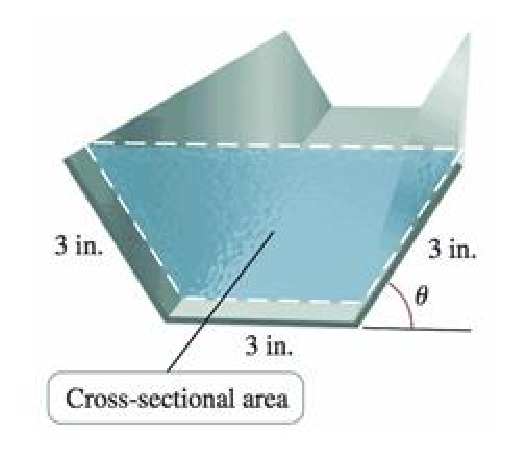
\includegraphics[scale=0.5]{gutter.eps}
\end{center}
\newpage
\end{CJK}
\end{document} 
